\section{First section}
Let's get writing. 

\section{Second section - this one has equations}
Writing equations is really easy, and you can refer back to them from any chapter (Equation \ref{1-equ:relativity}).
%
\begin{equation}
    \label{1-equ:relativity}
    E = mc^2
\end{equation}
%
You can also refer to figures. You can try to force figures to go in the text exactly where you place them, but most of the time it's better to place them right after you first mention it, make a \textit{suggestion} of its placement (here, top of page, bottom of page, or whole page) and let \LaTeX place it at the next available spot that doesn't interrupt flow too much. (see Figure \ref{1-fig:boats}). 
%
\begin{figure}[htbp]
    \centering
    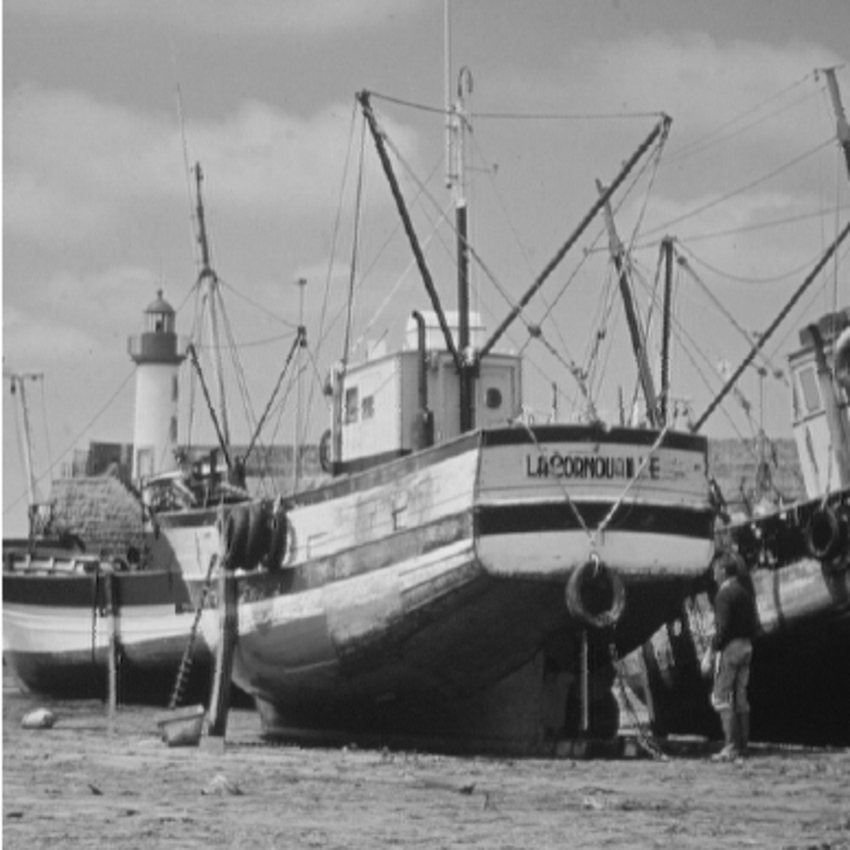
\includegraphics[width=0.75\linewidth]{figures/C1_general_intro/boat.png}
    \caption[This is a figure with an alternative caption]{This is a figure, with a long and descriptive caption. Figure captions should be able to stand on their own so they can get long. Maybe this was adapted from \citet{alexander_navigating_2016}, or maybe it relates to Equation \ref{1-equ:relativity} - who knows? All I know is that I don't want all this to appear in this Table of Figures.} 
    \label{1-fig:boats}
\end{figure}
%
You can even flow your text around a figure while writing and \LaTeX will stick the text blocks together like normal. 

\subsection{A subsection --- with acronyms!}
I may need to define some acronyms in the acronym document, like \ac{hab} and \ac{do}. Then I can talk about the effect of \ac{do} on \acp{hab} later on and everyone will know what I'm talking about. Did you notice that \ac{hab} was pluralised back there? What if I want a customised plural, like for \ac{ena}? I can do that --- the full version becomes \ac{ena} and the short version stays as \ac{ena}. I can also force capitalisation with \Ac{do}. 

\subsection{Here's another subsection --- with lists!}
\begin{enumerate}
    \item This is a list of things. I like to put lots of lists in my writing and I really with scientific writing would catch up with my genius.
    \item A list of aims maybe?
    \begin{enumerate}
        \item Nested lists automatically choose appropriate letters
        \item And always look nice
        \begin{itemize}
            \item And you can nest itemised lists and well.
            \item That's...
        \end{itemize}
        \item Super...
    \end{enumerate}
    \item Neat!
\end{enumerate}

\section{Primary aims and structure of this thesis}
The primary aims of this thesis were to....

\textbf{Chapter \ref{chap:1st-data}} aimed to...

\textbf{Chapter \ref{chap:2nd-data}} aimed to...

\textbf{Chapter \ref{chap:3rd-data}} aimed to...

Finally, \textbf{Chapter \ref{chap:gen-disc}} aimed to...
